\documentclass{SeminarV2}

\usepackage[latin1]{inputenc}
\usepackage{amssymb,amsmath,array}
\usepackage{graphicx}
\usepackage{placeins}


%***********************************************************************
% !!!! IMPORTANT NOTICE ON TEXT MARGINS !!!!!
%***********************************************************************
%
% Please avoid using DVI2PDF or PS2PDF converters: some undesired
% shifting/scaling may occur when using these programs
% It is strongly recommended to use the DVIPS converters.
%
% Check that you have set the paper size to A4 (and NOT to letter) in your
% dvi2ps converter, in Adobe Acrobat if you use it, and in any printer driver
% that you could use.  You also have to disable the 'scale to fit paper' option
% of your printer driver.
%
% In any case, please check carefully that the final size of the top and
% bottom margins is 5.2 cm and of the left and right margins is 4.4 cm.
% It is your responsibility to verify this important requirement.  If these margin requirements and not fulfilled at the end of your file generation process, please use the following commands to correct them.  Otherwise, please do not modify these commands.
%
\voffset 0 cm \hoffset 0 cm \addtolength{\textwidth}{0cm}
\addtolength{\textheight}{0cm}\addtolength{\leftmargin}{0cm}

%***********************************************************************
% !!!! USE OF THE SeminarV2 LaTeX STYLE FILE !!!!!
%***********************************************************************
%
% Some commands are inserted in the following .tex example file.  Therefore to
% set up your Seminar submission, please use this file and modify it to insert
% your text, rather than staring from a blank .tex file.  In this way, you will
% have the commands inserted in the right place.

% Edited by Martin Bogdan.

\begin{document}
%style file for Seminar manuscripts
\title{Computational Mechanisms of Sensorimotor Control}

%***********************************************************************
% AUTHORS INFORMATION AREA
%***********************************************************************
\author{Maximilian Joas$^1$ 
%
% Optional short acknowledgment: remove next line if non-needed
%\thanks{This is an optional funding source acknowledgement.}
%
% DO NOT MODIFY THE FOLLOWING '\vspace' ARGUMENT
\vspace{.3cm}\\
%
% Addresses and institutions (remove "1- " in case of a single institution)
University of Leipzig  - Department of Computer Science \\
Augustusplatz 10, 04109 Leipzig  - Germany\\}

%
% Remove the next three lines in case of a single institution

%***********************************************************************
% END OF AUTHORS INFORMATION AREA
%***********************************************************************

\maketitle

\begin{abstract}
	Inherent problems in sensorimotor control impair our ability to perform movements and react to our environment. Even though these problems are present sensoric and motoric ability of humans are outstanding. This is due to the fact that several computational mechanisms are used. Multisensory integration and forward models are such mechanisms that are also supported by evidence.

\end{abstract}

\section{Introduction}

The human ability to perform complex motor task and react is outstanding even in the face of several inherent problems in motor control. Computational strategies to overcome these problems are subject of this paper.
\subsection{Problems in Motor Control}
There are several problems for the motor system on order to perform skilled and efficient movements. The main problems are nonlinearity, nonstationarity, delays, redundancy, uncertainty,
and noise\cite{franklin2011computational}. This paper will shortly describe delays, noise and uncertainty and will present selected strategies how the sensorimotor system deals with these issues.
\subsubsection{Noise}
Noise is always present in the nervous system and influences sensory pathways as well as motoric pathways\cite{faisal2008noise}. Noise occurs at all stages of sensorimotor control,
from sensory processing to planning and to the execution of motor commands. Sensory noise is responsible for variability in estimating both internal states of the body and external states of the world. Noise also limits the ability to plan movements which leads 
to variability in movement endpoints \cite{gordon1994accuracy} \cite{vindras1998frames}. Furthermore it accounts for neuronal variability of
cortical neurons that can predict future kinematic variability in
reaching \cite{churchland2006central}. Additionally, variability of movements
can arise due to noise in motor commands \cite{van2009motor}. Importantly, the noise in motor commands seems to
increase with the level of the motor command \cite{jones2002sources} \cite{slifkin1999noise}. This is called signal-dependent noise
%t is your responsibility to verify this important requirement.  If these margin requirements and not fulfilled at the end of your file generation process, please use the commands at the beginning of the SeminarV2.tex file to correct them.  Otherwise, please do not modify these commands.
\subsubsection{Delays}
There are delays in every stage of our sensorimotor system, starting from the
delay in receiving afferent sensory information, to the delay in the neuromuscular system when executing efferent motor commands. Feedback of sensory information is contemplated by delays that are arising from receptor dynamics and conduction delays on nerve fibers and synaptic relays. These delays vary for different sensory modalities (e.g longer for hearing than for proprioception), but are around 100 milliseconds.
 Therefore, we effectively live in the
past, with the control systems only having access to outdated information about the external state of the environment  and internal state of the body \cite{franklin2011computational}.
\subsubsection{Uncertainty}
Uncertainty refers to the incomplete knowledge either with regard to
the state of the environment or of the task or rewards one could receive.
Among noise and delays, there are many other sources of uncertainty;
for example, uncertainty can be caused by limitations in receptor density
and the representation of an analog world with the digital neural
code \cite{franklin2011computational}.  The inherent ambiguity in
sensory processing is also a source for uncertainty; for instance when a
three-dimensional world is projected onto the two-dimensional 
retina \cite{yuille2006vision}.\newline
\newline
When reflecting on all that problems one might wonder how humans are not total helpless in day to day life or how it is even possible to perform motor tasks at a high level. Therefore humans can apply several mechanisms to overcome the described difficulties.


\section{Multisensory Integration}
Multisensory integration helps us to deal with uncertainty
and noise. Distinct sensory modalities can represent the
same information about the state of our body or the state
of the external world (e.g., auditory and visual location of
a noise source). When these different modalities are
experimentally put in conflict, for example by
mismatching the vision and sound of a human speaking,
the percept is something intermediate between the
percept of each input alone \cite{mcgurk1976hearing}. Even for normal sensory inputs, our sensory
system is variable and can have biases. Because of that,
the estimates from distinct modalities are not likely to be
equal. Within the Bayesian framework, we can ask what
is the most likely state of the world which showed the
multiple sensory inputs. Such a Bayesian model predicts
that a scalar estimate from two different modalities, such
as the visual and haptic size of a held object, should be
weighted and averaged to calculate an optimal estimate.
Most importantly, the weighting of each modality
should depend on its reliability, with the more reliable
stimuli contributing more to the final estimate. This kind
of model is supported by experimental studies of size
estimation from visual and haptic cues \cite{ernst2002humans}, location from visual and auditory cues \cite{kording2007causal}, and has been suggested to explain
ventriloquism \cite{alais2004ventriloquist}. The study by Ernst
and Banks will be explained in the following.

\subsection{Visual Haptic Integration}
In order to examine how examine if humans combine two sensory stimuli weighted by the reliability of the stimulus Ernst and Banks manipulated put the visual and haptic size of an object into conflict. Subjects were presented two objects: one comparison object which had always the same size (50 mm optic and visual) another object where the visual size and haptic size differed by -6 to +6 mm. The subjects had to chose which object was taller. In order to examine the weighting of the two stimuli different levels of noise were added to the visual stimulus.


\begin{figure}
	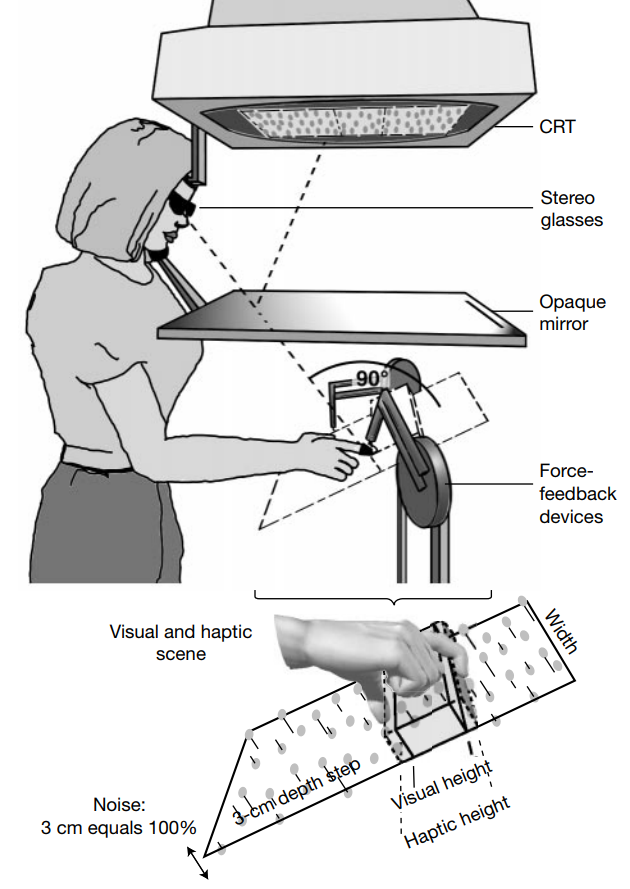
\includegraphics[width=0.65\linewidth]{erns_new.png}

	
	\caption{Experimental Setup: a, "Observers viewed the refection of the visual stimulus,
		presented on a cathode ray tube (CRT) binocularly in a mirror. The haptic stimulus was presented with two PHANToM force-feedback devices, one each
		for the index finger and thumb" \cite{ernst2002humans}.}
	\label{fig:boat1}
\end{figure}




\FloatBarrier


\subsubsection{Conclusion Study}
The more noise was added on the visual signal the more weight was given to the haptic size of the object. The weights of the stimuli were approximately mathematical optimal.This means using maximum likelihood estimation  This is an estimation where the weights W of two stimuli X\textsubscript{visual} and  X\textsubscript{haptic}, are calculated according to their variance $\sigma^2$: $\Theta$ = W $\cdot$X\textsubscript{visual} + (1-W) $\cdot$X\textsubscript{haptic} with  W = $\sigma^2$\textsubscript{haptic} / ( $\sigma^2$\textsubscript{haptic} + $\sigma^2$\textsubscript{visual} )

\begin{figure}
	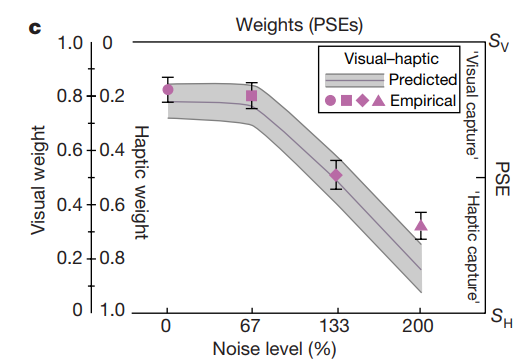
\includegraphics[width=0.9\linewidth]{erns_con.png}
	
	
	\caption{"Weights and PSEs. Abscissa represents the noise level, left
		ordinate represents visual weight (wV; haptic weight is 1 - wV) and right ordinate
		represents the PSEs relative to S V and S H. Purple symbols represent observed visual
		weights obtained from regression analysis of PSEs (equation 6) across D. Shaded area
		represents predicted weights expected from within-modality discrimination (a; equation
		(5)); its height represents predicted errors given the standard errors of the within-modality
		discrimination" \cite{ernst2002humans}.}
	\label{fig:reuslts}
\end{figure}
\FloatBarrier
\section{Forward Models}

While multisensory integration deals mainly with uncertainty forward models help to deal with delays (in addition to noise) \cite{franklin2011computational}. A forward model creates an instance of the motoric and sensoric system of the body. By doing so it works as a neural simulator that predicts the effects of motor commands \cite{franklin2011computational}. The concept of are forward model is difficult to validate experimentally. This is due to the fact that the output of the forward model is a prediction of a future state which is not measurable, but used to adjust motor commands \cite{mehta2002forward}. 
 However there are several studies supporting that estimations of the state of the body are made by sensory feedback as well as a forward model \cite{ariff2002real} \cite{nanayakkara2003saccade}. These studies used saccades (rapid eye movements between two points) to examine the existence of forward models
Subjects had to perform limb reaching movements and simultaneously track their limb position with their eyes. Thereby a it was found, that the saccades moved to a position 196 ms in advance of the limb position \cite{ariff2002real} . When disturbing the arm position it could be shown that saccades were initially suppressed for 100 ms after the disturbance. After the disturbance a recalculation followed and the eyes moved to a predicted position 150 ms before the hand. This suggest that the model has access to an efferent copy. The recalculation however was incorrect when the perturbation also changed the environment (for example by adding a resistive field). So subjects could not correctly predict their future limb position. This leads to the conclusion that sensory feedback and a model of the external world is used to predict a future outcome. When the model of the external world was wrong, the prediction was also not correct. In cases were there was time to learn the changes in the environment the model eventually performed correct predictions again \cite{nanayakkara2003saccade} . \newline

Prediction can be used for perception as well as for estimating the state of the body. More precise, sensory
prediction can be done by predicting the state of the
body and using this sensory prediction to cancel out the sensory
effects of movements (re-afference) \cite{franklin2011computational}.
This cancellation of self-generated sensory
feedback can be implemented to enhance the detection of sensory information that comes from the external world \cite{wolpert2001motor}. 

Another piece of evidence for this theory is that tickling yourself is way less ticklish than externally generated tickle. I order to distinguish between the self-generated movement to perform the tickle and the tactile sensation on the skin robotic manipulation was used. This was done by adding short delays or small changes to the movement. After manipulating the self generated tickle, the sensation became more ticklish \cite{blakemore1999spatio}. This shows that the prediction of our system which are used in sensory perception are highly exact temporally and spatially. 
A similar effect could be shown in force generation. Self-generated forces are perceived weaker than externally-generated forces.\cite{franklin2011computational}. Additionally, the idea of an efference copy that predicts the sensory input of a movement and removes the this prediction from the sensory perception is supported by the study of self-generated head movements. Thereby the predicted cancellation signal is subtracted but the vestibular nuclei \cite{roy2001selective}\cite{cullen2004signal} .
 
 

\section{Outlook}

Since this paper only contemplated a few selected mechanisms other principles should be shortly mentioned as well should be thought about possible applications of those computational mechanisms. A very powerful strategy is learning. Learning deals with non-linearity, non-stationarity and delays. Optimal control theory is also worth mentioning, since it is the only strategy that deals with redundancy. This is done by optimizing the costs of a movement\cite{franklin2011computational}. Costs can be anything from the loss of a desired position to energetic costs \cite{franklin2011computational}. \newline
Although the material presented in this paper is mostly basic research, one could think about applications in robotics. The application could be especially interesting, because the computational principles used by humans could be implemented easier than other neurobionic ideas.



 






% ****************************************************************************
% BIBLIOGRAPHY AREA
% ****************************************************************************

\begin{footnotesize}
\bibliography{own.bib}
\bibliographystyle{unsrt}
% IF YOU DO NOT USE BIBTEX, USE THE FOLLOWING SAMPLE SCHEME FOR THE REFERENCES
% ----------------------------------------------------------------------------

% ----------------------------------------------------------------------------

% IF YOU USE BIBTEX,
% - DELETE THE TEXT BETWEEN THE TWO ABOVE DASHED LINES
% - UNCOMMENT THE NEXT TWO LINES AND REPLACE 'Name_Of_Your_BibFile'


%\bibliography{Name_Of_Your_BibFile}

\end{footnotesize}

% ****************************************************************************
% END OF BIBLIOGRAPHY AREA
% ****************************************************************************

\end{document}
